\begin{figure}[H]
\begin{tabular}{@{}c@{}c@{}}
\begin{subfigure}[b]{0.4\textwidth}
\begin{center}
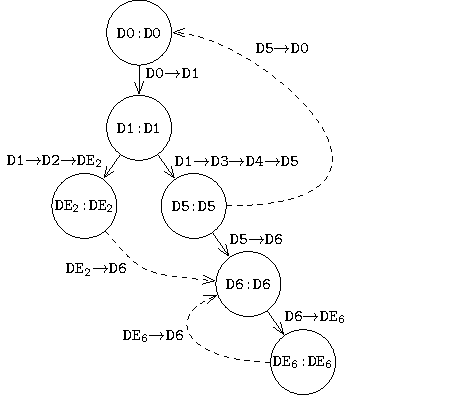
\includegraphics[scale=1]{chapters/figures/figClistDeconsProductCfg.pdf}
\end{center}
\caption{\label{fig:clistdeconsproductcfg} Decons-PCFG}
\end{subfigure}%
&
\begin{subfigure}[b]{0.6\textwidth}
\begin{center}
\begin{footnotesize}
\renewcommand{\arraystretch}{1.4}
\begin{tabular}{|c|l|}
\hline
{\bf PC-Pair} & \multicolumn{1}{c|}{\bf Invariants} \\
\hline
\hline
% \multirow{2}{*}{(\ddpc{0}{0})} &
% \Tstrut $\circled{\scriptsize P1} \  \fdv{l} = \sdv{l}$ \\
% & \Tstrut $\circled{\scriptsize P2} \  \fdv{\mem{}} = \mem{}$ $\circled{\scriptsize P3} \  \sdv{\mem{}} = \mem{}'$ \\
% \hline
\multirow{3}{*}{\shortstack[c]{(\ddpc{0}{0}) \\ (\ddpc{1}{1})}} & \Tstrut $\circled{I1} \ \fdv{l} = \sdv{l}$ \\
& \Tstrut $\circled{I2} \  \fdv{\mem{}} = \mem{}$ \\
& $\circled{I3} \  \sdv{\mem{}} = \mem{}'$ \\
\hline
\multirow{2}{*}{(\ddpc{5}{5})} &
\Tstrut $\circled{I4} \  \fdv{val} = \sdv{val}$ \\
& \Bstrut $\circled{I5} \  \structPointer{\fdv{l}}{\fdv{\mem{}}}{lnode}{next} = \structPointer{\sdv{l}}{\sdv{\mem{}}}{lnode}{next}$ \\
\hline
\multirow{2}{*}{(\ddpc{6}{6})} &
\Tstrut $\circled{I6} \  \fdv{val} = \sdv{val}$ \\
& \Tstrut \Bstrut $\circled{I7} \  \fdv{tail} = \sdv{tail}$ \\
\hline
\Tstrut (\ddpc{E_2}{E_2}) &
\multirow{2}{*}{$\circled{E} \   \fdv{ret} = \sdv{ret}$} \\
\Bstrut (\ddpc{E_6}{E_6}) & \\
\hline
\end{tabular}
\end{footnotesize}
\end{center}
\caption{\label{fig:clistdeconsproductcfginvs} Invariants Table}
\end{subfigure}%
\\
\end{tabular}
\caption{\label{fig:clistdeconsproductcfgandinvs} Decons-PCFG and invariants table for the deconstruction programs of \lifted{list}{\mem{}}{lnode}{\cv{l}} and \lifted{list}{\mem{}'}{lnode}{\cv{l}} respectively.}
\end{figure}